\documentclass[12pt]{extarticle}

% meta
\title{Отчет о практическом задании \\ <<Ансамбли алгоритмов. Веб-сервер. Композиции алгоритмов для решения задачи регрессии>>.\\[6mm] \large Практикум 317 группы, ММП ВМК МГУ.}
\author{Алексеев Илья Алексеевич.}
\date{Декабрь 2022.}

\usepackage[warn]{mathtext}
\usepackage[T2A]{fontenc}			% кодировка
\usepackage[utf8]{inputenc}			% кодировка исходного текста
\usepackage[english,russian]{babel}	% локализация и переносы
\usepackage{indentfirst}
\usepackage{csquotes}
\usepackage[bibstyle=gost-numeric, sorting=none]{biblatex}
\addbibresource{biblio.bib}

% page settings
\usepackage[left=1.8cm,right=1.8cm,
    top=1.8cm,bottom=1.8cm,bindingoffset=0cm]{geometry}

\usepackage{graphicx, hyperref, xcolor}
\hypersetup{
    colorlinks=true,
    linkcolor=teal,
    filecolor=magenta, 
    urlcolor=blue,
    citecolor=olive,
    pdftitle={GD},
    pdfpagemode=FullScreen,
    linktoc=all
    }

\usepackage{wrapfig,caption}

% figures
\usepackage{caption}
\usepackage{subcaption}
\usepackage{floatrow}
\floatsetup{heightadjust=object}

% math
\usepackage{amsmath,amsfonts,amssymb,amsthm,mathtools,esint,eucal}

\newcommand{\R}{\mathbb{R}}
\newcommand{\A}{\mathcal{A}}
\DeclareMathOperator{\var}{\text{Var}}
\DeclareMathOperator{\cov}{\text{Cov}}

\begin{document}

\maketitle

\tableofcontents

\newpage

\section{Введение.}

В рамках данного практического задания были реализованы методы линейного ансамблирования деревьев: Random Forest и Gradient Boosting. Изучена зависимость точности предсказаний и время обучения в зависимости от размера подпространства в методе случайных подпространств, ограничений на глубину деревьев, числа деревьев и величины шага спуска. Реализованные алгоритмы обёрнуты в web-приложение.

\subsection{Random Forest.}

Алгоритм \textit{Random Forest} \cite{lin} в рамках задачи регрессии он состоит в том, чтобы обучить $N$ деревьев и посчитать среднее арифметическое их предсказаний.

Пусть $b_n:\R^d\to\R,\ n=\overline{1,N}$ -- решающие деревья для задачи регрессии. Тогда Random Forest делает предсказание как
\begin{equation*}
    a_N(x)={1\over N}\sum_{i=1}^Nb_n(x).
\end{equation*}

Для алгоритма $a_N(x)$ variance-компонента в разложении на смещение и разброс записывается следующим образом:
\begin{equation}\label{eq:var}
    \var[a_N]={1\over N}\var[b_i]+{N(N-1)\over N^2}\cov(b_i,b_j).
\end{equation}
То есть разброс Random Forest состоит из разброса одного дерева, поделённого на их число, плюс ковариация всех деревьев. Это значит, что если одновременно снижать коррелированность (зависимость, похожесть) деревьев и увеличивать их число, разброс ансамбля будет минимизироваться.

Корреляцию между деревьями можно уменьшить, например, двумя способами: 1) обучать каждое дерево не на всём датасете, а на подвыборке, сформированной с помощью взятия с возвращением (\textit{bootstrap}); 2) обучать каждое дерево не по всем признакам, а по случайно выбранному подмножеству (\textit{метод случайных подпространств}).

\subsection{Gradient Boosting.}

Алгоритм \textit{Gradient Boosting} следующий \cite{adv}. Первый базовый алгоритм обучается предсказывать целевую переменную $y\in\R^\ell$, где $\ell$ -- размер выборки. Второй базовый алгоритм обучается на ошибку первого алгоритма, т.е. вектор $s^{(1)}\in\R^\ell$ с компонентами $s_i^{(1)}=y_i-b_1(x_i)$. $(n+1)$-ый базовый алгоритм обучается предсказывать $s_i^{(n)}\in\R^\ell$ с компонентами $s_i^{(n)}=y_i-a_n(x_i)$, где $a_n$ -- ансамбль из $n$ алгоритмов. Его предсказание строится следующим образом:
\begin{equation*}
    a_n(x)=a_{n-1}+\alpha w_nb_n(x),
\end{equation*}
где $\alpha$ --- гиперпараметр метода, $w_n$ -- вес. Веса подбираются как решение оптимизационной задачи:
\begin{equation*}
    w_n=\arg\min_w\sum_{i=1}^\ell L(y_i,a_{n-1}+wb_n(x_i))^2.
\end{equation*}

Величина $s^{(n)}$ имеет смысл направления убывания ошибки предсказания, поэтому когда мы обучаем $b_n$, мы ищем аппроксимацию антиградиента, а когда добавляем обученный $b_n$ в ансамбль, мы делаем шаг градиентного спуска в пространстве предсказаний $\R^\ell$.

\section{Эксперименты.}

Из датасета \textit{House Sales in King County, USA} убран признак \texttt{id}, принимающий значения типа \texttt{7129300520} или \texttt{2487200875}. Признак \texttt{date} формата \texttt{\%Y\%m\%dT000000} заменён на три признака \texttt{year}, \texttt{month}, \texttt{day}. Затем признак \texttt{year} заменён на \texttt{year\_2014} и \texttt{year\_2015} с помощью OneHot кодирования. Признаки \texttt{month} и \texttt{day} преобразованы в \texttt{month\_sin}, \texttt{month\_cos}, \texttt{day\_sin}, \texttt{day\_cos} как циклические признаки. Весь датасет случайным образом поделён на три выборки: обучающую, валидационную и тестовую (в соотношении 3:1:1).

\subsection{Размер случайного подпространства.} \label{sec:subspacesize}

В данном эксперименте были рассмотрены значения параметра \texttt{subspace\_size} (доля признаков, используемых для обучения отдельного дерева) в отрезке $[0.1, 1]$ с шагом $0.1$. Для каждого значения были обучены модели Random Forest и Gradient Boosting и замерена ошибка RMSE на валидации. Эксперимент повторён пять раз, значения ошибки усреднены (рис. \ref{fig:subspacesize}). Использовались параметры из табл. \ref{tbl:supspacesize}.

\begin{figure}[!htb]
     \caption{Значения RMSE и время обучения в зависимости от доли признаков, выбираемых для обучения деревьев в ансамблях деревьев.}
     \centering
     \begin{subfigure}[t]{0.48\linewidth}
        \caption{Random Forest.}
        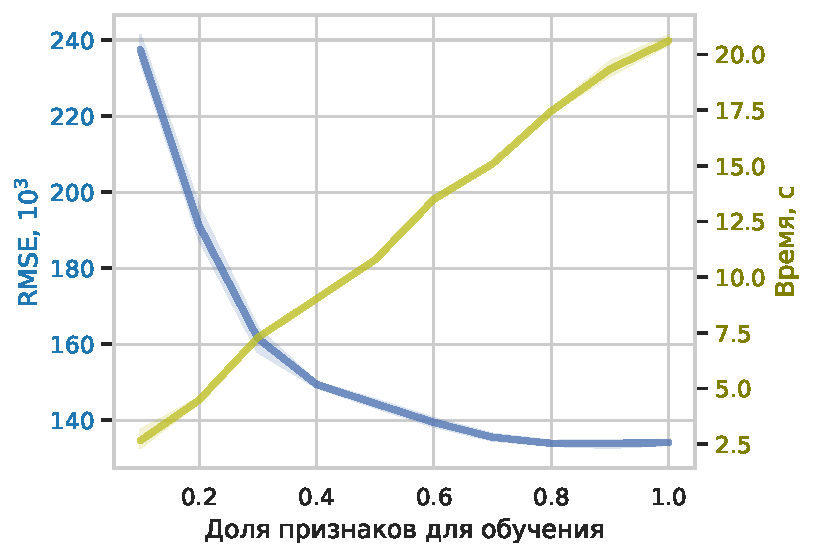
\includegraphics[width=1\linewidth]{pics/feature_fraction.pdf}
        \label{fig:feature_fraction}
     \end{subfigure}
     \begin{subfigure}[t]{0.48\linewidth}
        \caption{Gradient Boosting.}
        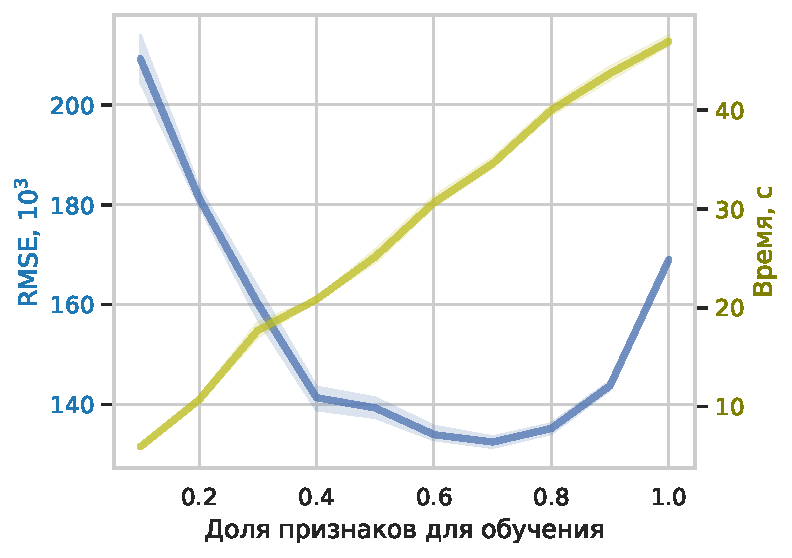
\includegraphics[width=1\linewidth]{pics/gbfeature_fraction.pdf}
        \label{fig:gbfeature_fraction}
     \end{subfigure}
     \label{fig:subspacesize}
\end{figure}

\begin{wraptable}[7]{r}{0.3\linewidth}
    \vspace{-5mm}
    \caption{Параметры эксперимента \ref{sec:subspacesize}.}
    \label{tbl:supspacesize}
    \begin{tabular}{c|c|c}
        Параметр & RF & GB \\
        \hline
        \texttt{n\_estimators} & 200 & 200\\
        \texttt{max\_depth} & 50 & 50\\
        \texttt{learning\_rate} & --- & 0.05\\
    \end{tabular}
\end{wraptable} 

На рис. \ref{fig:feature_fraction} ошибка предсказания уменьшается с ростом параметра вплоть до значения параметра $0.8$, затем выходит на плато. Это можно интерпретировать следующим образом: 1) малое число признаков не дает достаточное количество информации для точного предсказания; 2) полный набор признаков не улучшает качество предсказания, так как делает деревья коррелированными и вносит вклад во второе слагаемое в формуле \eqref{eq:var}.

На рис. \ref{fig:gbfeature_fraction} ошибка предсказания уменьшается с ростом параметра вплоть до значения $0.7$, а затем в отличие от Random Forest резко растет. Значит, для аппроксимации антиградиента излишняя точность приводит к ухудшению бустинга.

Время обучения для обеих моделей имеет одинаковую зависимость: оно прямо пропорционально параметру, что объясняется тем, что увеличение признакового пространства увеличивает время поиска оптимального признака, по которому производится деление в узлах дерева. 

\subsection{Максимальная глубина дерева.} \label{sec:maxdepth}

В данном эксперименте были рассмотрены значения параметра \texttt{max\_depth} (ограничение на максимальную глубину дерева в ансамбле). Для модели Random Forest рассмотрены значения в отрезке $[10, 190]$ с шагом $20$. Для модели Gradient Boosting -- значения $[1,10]$ и $20,30$. Для каждого значения замерена ошибка RMSE на валидации. Эксперимент повторён пять раз, значения ошибки усреднены (рис. \ref{fig:maxdepth}).

\begin{figure}[!htb]
     \caption{Значения RMSE и время обучения в зависимости от ограничения на глубину дерева в ансамблях деревьев.}
     \centering
     \begin{subfigure}[t]{0.48\linewidth}
        \caption{Random Forest.}
        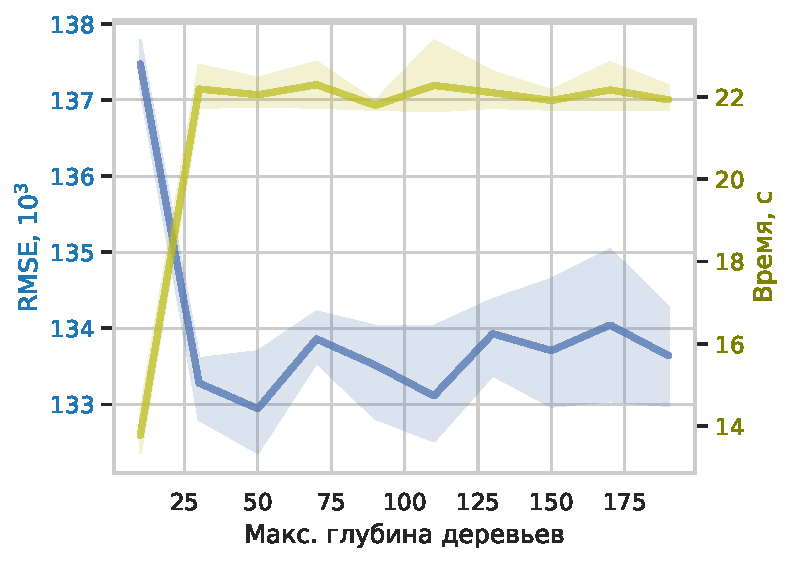
\includegraphics[width=1\linewidth]{pics/max_depth.pdf}
        \label{fig:max_depth}
     \end{subfigure}
     \begin{subfigure}[t]{0.48\linewidth}
        \caption{Gradient Boosting.}
        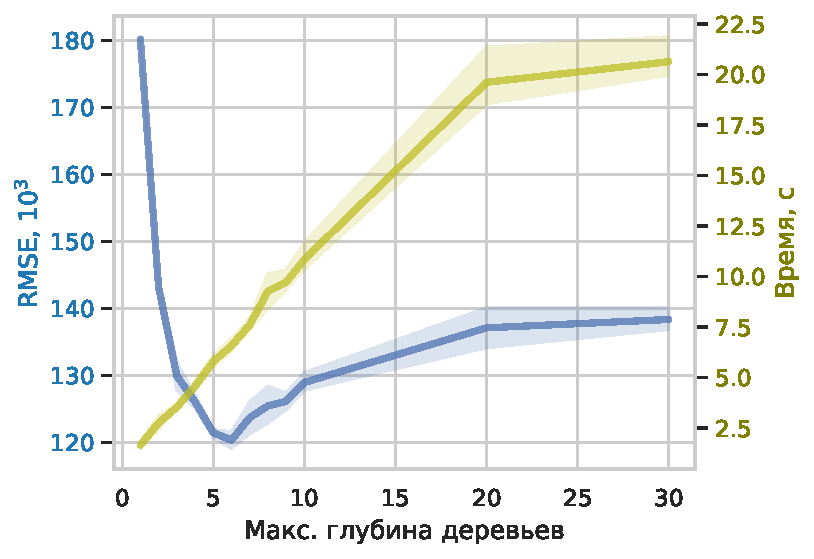
\includegraphics[width=1\linewidth]{pics/gbmax_depth.pdf}
        \label{fig:gbmax_depth}
     \end{subfigure}
     \label{fig:maxdepth}
\end{figure}

\begin{wraptable}[7]{r}{0.3\linewidth}
    \vspace{-5mm}
    \caption{Параметры эксперимента \ref{sec:maxdepth}.}
    \label{tbl:maxdepth}
    \begin{tabular}{c|c|c}
        Параметр & RF & GB \\
        \hline
        \texttt{n\_estimators} & 200 & 200 \\
        \texttt{subspace\_size} & 0.8 & 0.7 \\
        \texttt{learning\_rate} & --- & 0.05\\
    \end{tabular}
\end{wraptable} 

На рис. \ref{fig:max_depth} ошибка предсказания уменьшается при изменении глубины с $10$ до $30$, затем выходит на плато. Заметим, что отдельные деревья в большинстве не используют всю предоставленную глубину, т.к. время обучения не меняется с ростом параметра.

Полупрозрачная область около линии -- это $95$-доверительный интервал, он характеризует разброс результатов пяти экспериментов. Визуально может показаться, что разброс велик, но на самом деле он составляет не более $\pm10^3$, что в сравнении с ошибкой RMSE порядка $10^5$ незначительно. Это подтверждает, что отдельные деревья не строятся во всю глубину.

На рис. \ref{fig:gbmax_depth} ошибка предсказания уменьшается при изменении глубины с $1$ до $6$, затем растёт и выходит на плато. Увеличение времени обучения говорит о том, что отдельные деревья строятся в полную глубину. Значит, 1) существует оптимальная глубина; 2) выводы, аналогичные Random Forest.

\subsection{Число деревьев.} \label{sec:nestimators}

В данном эксперименте были рассмотрены значения параметра \texttt{n\_estimators} (число деревьев в ансамбле) в отрезке $[50, 1000]$ с шагом $50$. Для каждого значения были обучены модели Random Forest и Gradient Boosting и замерена ошибка RMSE на валидации. Эксперимент повторён четыре раза, значения ошибки усреднены (рис. \ref{fig:nestimators}). Использовались параметры из табл. \ref{tbl:nestimators}.

\begin{figure}[!htb]
     \caption{Значения RMSE и время обучения в зависимости от числа деревьев в ансамбле.}
     \centering
     \begin{subfigure}[t]{0.48\linewidth}
        \caption{Random Forest.}
        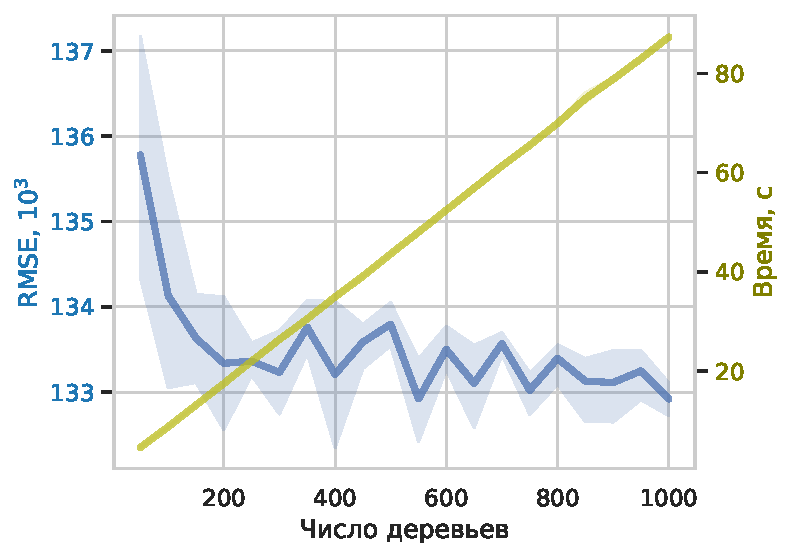
\includegraphics[width=1\linewidth]{pics/n_estimators.pdf}
        \label{fig:n_estimators}
     \end{subfigure}
     \begin{subfigure}[t]{0.48\linewidth}
        \caption{Gradient Boosting.}
        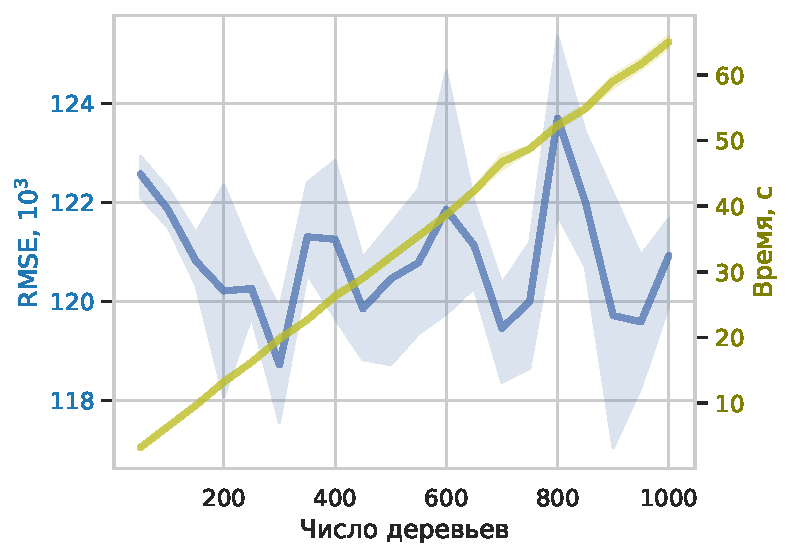
\includegraphics[width=1\linewidth]{pics/gbn_estimators.pdf}
        \label{fig:gbn_estimators}
     \end{subfigure}
     \label{fig:nestimators}
\end{figure}

\begin{wraptable}[7]{r}{0.3\linewidth}
    \vspace{-5mm}
    \caption{Параметры эксперимента \ref{sec:nestimators}.}
    \label{tbl:nestimators}
    \begin{tabular}{c|c|c}
        Параметр & RF & GB \\
        \hline
        \texttt{max\_depth} & 50 & 6 \\
        \texttt{subspace\_size} & 0.8 & 0.7 \\
        \texttt{learning\_rate} & --- & 0.05\\
    \end{tabular}
\end{wraptable} 

На рис. \ref{fig:n_estimators} ошибка предсказания уменьшается при изменении числа деревьев с $50$ до $200$, затем выходит на плато (отклоняется от тренда максимум на $\pm10^3$). Учитывая, что порядок изменяется на порядок (до тысячи), а ошибка предсказаний не увеличивается, можем сделать вывод, что число деревьев не приводит к переобучению.

На рис. \ref{fig:gbn_estimators} ошибка предсказания осциллирует около одного и того же значения, изменяясь незначительно. В сравнении с \ref{fig:n_estimators} значение ошибки меньше примерно на $10\%$, но разброс в два раза больше. Время обучения для обеих моделей имеет одинаковую зависимость: оно прямо пропорционально параметру, что объясняется тем, что увеличение числа деревьев увеличивает суммарное время обучения модели.

\subsection{Размер шага в Gradient Boosting.} \label{sec:lr}

\begin{wrapfigure}[16]{r}{0.5\linewidth}
    \vspace{-3mm}
    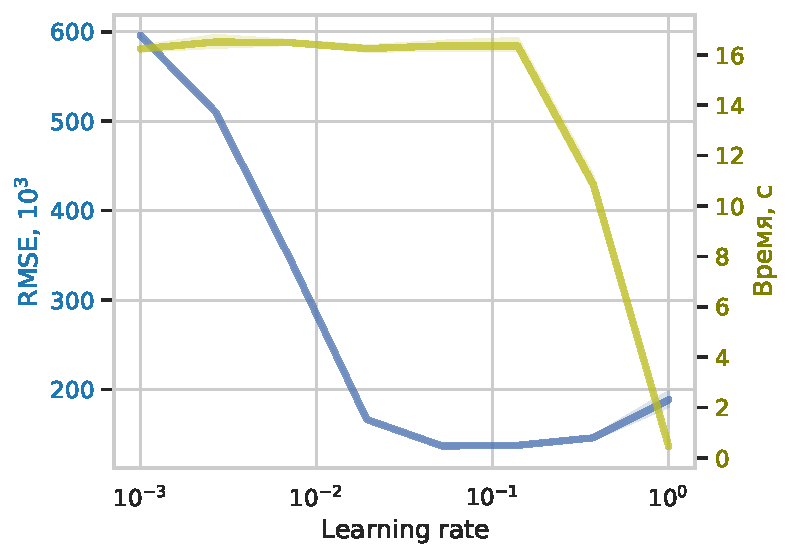
\includegraphics[width=1\linewidth]{pics/lr.pdf}
    \caption{Значения RMSE и время обучения модели Gradient Boosting в зависимости от шага.}
    \label{fig:lr}
    \centering
\end{wrapfigure}
В данном эксперименте были рассмотрены значения параметра \texttt{learning\_rate} (размер шага градиентного бустинга) на отрезке $[10^{-3}, 10^0]$, восемь значений из логарифмической сетки. Параметры брались из табл. \ref{tbl:supspacesize}. Для каждого значения была обучена модель Gradient Boosting и замерена ошибка RMSE на валидации. Эксперимент повторён пять раз, значения ошибки усреднены (рис. \ref{fig:lr}). Ошибка предсказания уменьшается при изменении параметра с $10^{-3}$ до $\approx5\cdot 10^-2$, затем выходит на плато и растет.

Поскольку Gradient Boosting является градиентными спуском в пространстве предсказаний, такое поведение ошибки объяснимо тем, что 1) малый шаг не позволяет спуску добраться до окрестности оптимума за отведённое число итераций; 2) большой шаг не позволяет спуску сойтись.

При больших значениях шага также резко снижается время обучения. Это объясняется тем, что окрестность оптимума успешно достигается самыми первыми деревьями и под большинство объектов ансамбль уже <<настроился>>. Остаётся часть объектов, предсказания для которых отличаются значительно. Их достаточно много, чтобы ошибка RMSE была высокой, и одновременно их достаточно мало, чтобы деревья могли делить их и уменьшать энтропию.

\section{Выводы.}

\begin{wraptable}[9]{r}{0.3\linewidth}
    % \vspace{-5mm}
    \caption{Оптимальные параметры.}
    \label{tbl:summary}
    \begin{tabular}{c|c|c}
        Параметр & RF & GB \\
        \hline
        \texttt{n\_estimators} & 200 & 200 \\
        \texttt{max\_depth} & 50 & 6 \\
        \texttt{subspace\_size} & 0.8 & 0.7 \\
        \texttt{learning\_rate} & --- & 0.05\\
    \end{tabular}
\end{wraptable} 

Линейные методы ансамблирования Random Forest и Gradient Boosting чувствительны к выбору параметров базовых алгоритмов. Чтобы избежать их коррелированности и излишней точности нужно подбирать размер случайного подпространства (раздел \ref{sec:subspacesize}). Метод Gradient Boosting требует строгое ограничение на высоту деревьев, в то время как Random Forest просто не использует доступную высоту (раздел \ref{sec:maxdepth}). Оба метода не деградируют при увеличении числа базовых алгоритмов (раздел \ref{sec:nestimators}). Размер шага существенно влияет на сходимость Gradient Boosting (раздел \ref{sec:lr}).

Оптимальные параметры к датасету \textit{House Sales in King County, USA} приведены в табл. \ref{tbl:summary}.

\printbibliography

\end{document}
